%!TEX root = ../LaTeX-cn.tex
\chapter{\LaTeX{}基础}
\section{第一份文稿}

编辑器的配置大概是需要讲解一下的,毕竟对于初学者来说是很头疼的事情。本手册就以\TeX Studio为例进行配置。首先你应该安装一个\TeX{} Live,它是完全免费的,网址:\url{http://tug.org/texlive/}.

虽然它体积较大,但是却是最一劳永逸、最不需要花时间取配置的方法,同时它大概也是功能支持最强的\LaTeX 发行版。

打开\TeX Studio后,选择选项$\rightarrow$ 设置\TeX Studio $\rightarrow$ 构建$\rightarrow$ 默认编译器,选择\xelatex{}. 这主要是基于中文文档编译的考虑,同时\xelatex 也能很好地编译英文文档。我建议始终使用它作为默认编译器。\dpar

之后你可以在窗口输入一篇小文档,并保存为tex扩展名的文件进行测试:
\begin{latex}
\documentclass{ctexart}
\begin{document}
    Hello, world!
    你好,世界!
\end{document}
\end{latex}

点击编译按钮生成,F7查看。生成的pdf在你的tex文件保存目录中。具体各行的含义我们会在后文介绍。

\section{认识\LaTeX}
\subsection{命令与环境}
\LaTeX 中的\co{命令}通常是由一个反斜杠加上命令名称,再加上花括号内的参数构成的(有的命令不带参数,例如:\latexline{TeX})。
\begin{latex}
\documentclass{ctexart}
\end{latex}

如果有一些选项是备选的,那么通常会在花括号前用方括号标出。比如:
\begin{latex}
\documentclass[a4paper]{ctexart}
\end{latex}

还有一种重要指令叫做\co{环境}。它被定义于控制命令\latexline{begin\{environment\}} 和\latexline{end\{environment\}}间的内容。比如:
\begin{latex}
\begin{document}
...内容...
\end{document}
\end{latex}

环境如果有备选参数,只需要写在\latexline{begin[...]\{name\}}这里就行。

注意:不带花括号的命令后面如果想打印空格,请加上\RED{一对内部为空的花括号}再键入空格。否则空格会被忽略。例如:\verb+\LaTeX{} Studio+.

\subsection{保留字符}

\LaTeX 中有许多字符有着特殊的含义,在你生成文档时不会直接打印。例如每个命令的第一个字符:反斜杠。单独输入一个反斜杠在你的行文中不会有任何帮助,甚至可能产生错误。\LaTeX 中的保留字符有:
\begin{center}
\texttt{\# \$ \% \^ \& \_ \{ \} \char92}
\end{center}

它们的作用分别是:
\begin{para}
\item[\#{}:] 自定义命令时,用于标明参数序号。
\item[\${}:] 数学环境命令符。
\item[\%{}:] 注释符。在其后的该行命令都会视为注释。如果在回车前输入这个命令,可以防止行末\LaTeX 插入一些奇怪的空白符。
\item[\^{}:] 数学环境中的上标命令符。
\item[\&{}:] 表格环境中的跳列符。
\item[\_{}:] 数学环境中的下标命令符。
\item[\{与\}:] 花括号用于标记命令的必选参数,或者标记某一部分命令成为一个整体。
\item[\char92{}:] 反斜杠用于开始各种\LaTeX 命令。
\end{para}

以上除了反斜杠外,均能用前加反斜杠的形式输出。即你只需要键入:
\begin{center}
\verb|\# \$ \% \^ \& \_ \{ \}|
\end{center}

唯独反斜杠的输出比较头痛,你可以尝试:
\begin{codeshow}
$\backslash$ \textbackslash
\texttt{\char92}
\end{codeshow}

其中命令\latexline{char[num]}是一个特殊的命令,使用环境需要是tt字体环境,用于输出USCII码对应的字符;92对应的即反斜杠。你也可以用\latexline{char`}后加字符的方式输出你想输出的命令,但需要包裹在\latexline{texttt}或者\latexline{ttfamily}内。如果想输出的字符是保留字符,需要再加一个反斜杠。
\begin{verbatim}
\texttt{\char`~} % 输出一个波浪线
\texttt{\char`\\} % 输出保留字反斜杠
\texttt{\char`@} % 实际上可直接输入@
\end{verbatim}

另外需要说明的是,上例提及的波浪线{\texttt{\~}}用来输出一个禁止在该处断行的空格,也不能够直接输出。尝试:
\begin{codeshow}
a $\sim$ b
a\~ b
a\~{} b
a\textasciitilde b
\end{codeshow}

\subsection{导言区}
任何一份\LaTeX{}文档都应当包含以下结构:
\begin{latex}
\documentclass[`\itshape options`]{doc-class}
\begin{document}
    ...
\end{document}
\end{latex}

其中,在语句\latexline{begin\{document\}}之前的内容称为\co{导言区}。导言区可以留空,以可以进行一些文档的准备操作。你可以粗浅地理解为:\RED{导言区即模板定义}。\dpar

文档类的参数doc-class和可选选项{\textit{options}}有\tref{tab:documentclass}取值:
\begin{table}[!htb]
    \centering
	\caption{文档类和选项}
	\label{tab:documentclass}
	\begin{tabular}{p{5em} @{\ -\ } p{24em}}
		\hline
		\multicolumn{2}{l}{\bfseries doc-class文档类\footnotemark} \\
		\hline
		article   & 科学期刊,演示文稿,短报告,邀请函。\\
		proc      & 基于article的会议论文集。\\
		report    & 多章节的长报告、博士论文、短篇书。\\
		book      & 书籍。\\
		slides    & 幻灯片,使用了大号Scans Serif字体。\\
		\hline
		\multicolumn{2}{l}{\bfseries\itshape options} \\
		\hline
		字体     & 默认10pt,可选11pt和12pt.\\
		页面方向 & 默认竖向portrait,可选横向landscape。\\
		纸张尺寸 & 默认letterpaper,可选用a4paper, b5paper等。\\
		分栏     & 默认onecolumn,还有twocolumn。\\
		双面打印 & 有oneside/twoside两个选项,用于排版奇偶页。article/report默认单面。\\
		章节分页 & 有openright/openany两个选项,决定是在奇数页开启新页或是任意页开启新页。注意article是没有chapter(``章'')命令的,默认任意页。\\
		公式对齐 & 默认居中,可改为左对齐fleqn;默认编号居右,可改为左对齐leqno。\\
		草稿选项 & 默认final,可改为draft,使行溢出的部分显示为黑块。\\
		\hline
	\end{tabular}
\end{table}

在本文中,多数的文档类提及的均为report/book类。如果有article类将会特别指明。其余的文档类不予说明。本手册排版即使用了report类。\dpar

在导言区最常见的是\co{宏包}的加载工作,命令形如:\latexline{usepackage\{package\}}。通俗地讲,宏包是指一系列已经制作好的功能``模块'',在你需要使用一些原生\LaTeX 不带有的功能时,只需要调用这些宏包就可以了。比如本文的代码就是利用\pkg{listings}宏包实现的。

宏包的具体使用将参在各部分内容说明中进行讲解。如果你想学习一个宏包的使用,按Win+R组合键呼出运行对话框,输入texdoc加上宏包名称即可打开宏包帮助pdf文档。例如:\verb|texdoc xeCJK|。

\footnotetext{此外还有\pkg{beamer}宏包定义的beamer文档类,常用于创建幻灯片。}

\subsection{错误的排查}
\label{subsec:debug}
在编辑器界面上,下方的日志是显示编译过程的地方。在你编译通过后,会出现这样的字样:
\begin{feai}
	\item {\qd{Errors错误}}:严重的错误。一般地,编译若通过了,该项是零。
	\item {\qd{Warnings警告}}:一些不影响生成文档的瑕疵。
	\item {\qd{Bad Boxes坏箱}\footnote{Box是\LaTeX{}中的一个特殊概念,具体将在\hyperref[sec:box]{这里}进行讲解。}}:指排版中出现的长度问题,比如长度超出(Overfull)等。后面的Badness表示错误的严重程度,程度越高数值越大。这类问题需要检查,排除Badness高的选项。
\end{feai}

你可以向上翻阅日志记录(即.log文件),来找到Warning开头的记录,或者Overfull/ Underfull开头的记录。这些记录会指出你的问题出在哪一行(比如line 1-2) 或者在pdf的哪一页(比如active [12]。注意,这个12表示计数器计数页码,而不是文件打印出来的真实页数)。此外你还需要了解:
\begin{feai}
	\item 值得指出的是,由于\LaTeX{}的编译原理(第一次生成aux文件,第二次再引用它),目录想要合理显示\qd{需要连续编译两次}。在连续编译两次后,你会发现一些Warnings会在第二次编译后消失。在\TeX Studio中,你可以只单击一次“构建并查看”,它会检测到文章的变化并自动决定是否需要编译两次。
	\item 对于大型文档,寻找行号十分痛苦。你需要学会合理地拆分tex文件,参阅\secref{sec:include}的内容。
\end{feai}

这里也推荐宏包\pkg{syntonly},在导言区加入它支持的\latexline{syntaxonly}命令,会只排查语法错误而不生成任何文档,这可以使你更快地编译。不过它似乎不太稳定,例如本文档可以正常编译,但是使用该命令时则会出错。

\subsection{文件输出}
\LaTeX{}的输出一般推荐pdf格式,由\LaTeX 直接生成dvi的方法并不推荐。

你在tex文档的文件夹下可能看到的其他文件类型:
\begin{tabbing}
	.sty{\hspace{2em}}\=宏包文件\\
	.cls	\> 文档类文件。\\
	.aux    \> 用于储存交叉引用信息的文件。因此,在更新交叉引用(公式编号、\\
	\> 大纲级别)后,需要编译两次才能正常显示。\\
	.log    \> 日志。记录上次编译的信息。\\
	.toc    \> 目录文件。\\
	.lof    \> 图形目录。\\
	.lot    \> 表格目录。\\
	.idx    \> 如果文档中包含索引,该文件用于储存索引信息。\\
	.ind	\> 索引记录文件。\\
	.ilg	\> 索引日志文件。\\
	.bib	\> \bibtex 参考文献数据文件。\\
	.bbl	\> \bibtex 生成的参考文献记录。\\
	.bst	\> \bibtex 模板。\\
	.blg	\> \bibtex 日志。\\
	.out	\> \texttt{hyperref}宏包生成的pdf书签记录。
\end{tabbing}

有时\LaTeX 的编译出现异常,你需要删除文件夹下除了tex以外的文件再编译。此外,在某些独占程序打开了以上的文件时(比如用Acrobat打开了pdf),编译可能出现错误。请在编译时确保关闭这些独占程序。

\section{标点与强调}
英文符号$|<>+=$一般用于数学环境中,如果在文本中使用,请在它们两侧加上“\$”。如果你在\LaTeX 中直接输入大于、小于号而不把它们放在数学环境中,它们并不会被正确地打印。你应该使用\latexline{textgreater}, \latexline{textless}命令。

在科技文章中,中文的句号也一般使用全角圆点“.”\footnote{这个标点是U+FF0E,称为“FULLWIDTH FULL STOP”。}而不是平常的“。”,也不是正常的英文句点“.”。这个符号很难正常输入;你可以先输入正常句点,最后再替换。

\subsection{引号}
英文单引号并不使用两个\verb|'|符号组合。左单引号是重音符\verb|`|(键盘上数字1左侧),而右单引号是常用的引号符。英文中,\RED{左双引号就是连续两个重音符}。

英文下的引号嵌套需要借助\latexline{thinspace}命令分隔,比如:
\begin{verbatim}
``\thinspace`Max' is here.''
\end{verbatim}

中文下的单引号和双引号你可以用中文输入法直接输入。

\subsection{破折、省略号与短横}
英文的短横分为三种:
\begin{feai}
\item 连字符:输入一个短横:\verb|-|,效果如daughter-in-law
\item 数字起止符:输入两个短横:\verb|--|,效果如:page 1--2
\item 破折号:输入三个短横:\verb|---|,效果如:Listen---I'm serious.
\end{feai}

中文的破折号你也许可以直接使用日常的输入方式。中文的省略号同样。但是注意,英文的省略号使用\latexline{ldots}这个命令而不是三个句点。

\subsection{强调:粗与斜}
\LaTeX 中专门有个叫做\latexline{emph\{text\}}的命令,可以强调文本。对于通常的西文文本,上述命令的作用就是斜体。如果你对一段已经这样转换为斜体的文本再使用这个命令,它就会取消斜体,而成为正体。

西文中一般采用上述的斜体强调方式而不是粗体,例如在说明书名的时候可能就会使用以上命令。关于字体的更多内容参考\hyperref[sec:font]{字体}这一节。

\subsection{下划线与删除线}
\LaTeX 原生提供的\latexline{underline}命令简直烂的可以,建议你使用\pkg{ulem}宏包下的\texttt{uline}命令代替,它还支持换行文本。\pkg{ulem}宏包还提供了一些实用命令:

\begin{codeshow}
\uline{下划线} \\
\uuline{双下划线} \\
\dashuline{虚下划线} \\
\dotuline{点下划线} \\
\uwave{波浪线} \\
\sout{删除线} \\
\xout{斜删除线}
\end{codeshow}

需要注意的是,\pkg{ulem}宏包重定义了\latexline{emph}命令,\RED{使得原来的加斜强调变成了下划线、原来的两次强调就取消强调变成了两次强调就双下划线}。通过宏包的normalem选项可以取消这个更改:\verb|\usepackage[normalem]{ulem}|。

\subsection{其他}
角度符号或者温度符号需要借助数学模式\verb|$...$|输入:

\begin{codeshow}
$30\,^{\circ}$三角形 \\
$37\,^{\circ}\mathrm{C}$
\end{codeshow}

欧元符可能需要用到\pkg{textcomp}宏包支持的\latexline{texteuro}命令。

其次是千位分隔位,比如\verb|1\,000\,000|。如果你不想它在中间断行就在外侧再加上一个\latexline{mbox}命令:\latexline{mbox\{1\char`\\,000\char`\\,000\}}。

再次是注音符号,比如\^o,也常用于拼音声调,参考\hyperref[app:phonetic]{注音符号表}部分的附录内容。如果你想输入音标,请使用tipa宏包\footnote{tipa会重定义\latexline{!}命令,因此请使用\latexline{negthinspace}代替;或在\pkg{xeCJK}与\pkg{amsmath}宏包前加载,并使用safe选项。具体可以参见本手册的 Head.tex 文件。},同样参考附录A。

最后,介绍\pkg{hologo}宏包,它可以输出许多\TeX 家族标志。其实\LaTeX 原生自带了\latexline{LaTeX}, \latexline{TeX}等命令。而hologo宏包支持的命令有:

\begin{codeshow}
% 大写H表示符号的首字母也大写
\hologo{XeLaTeX} \Hologo{BibTeX}
\end{codeshow}

\section{格式控制}
首先了解一下\hologo{LaTeX}的长度单位:
\begin{fead}
  \item[pt] point,磅。\label{sec:length}
  \item[pc] pica。1pc=12pt,四号字大小
  \item[in] inch,英寸。1in=72.27pt
  \item[bp] bigpoint,大点。1bp=$\frac{1}{72}$in
  \item[cm] centimeter,厘米。1cm=$\frac{1}{2.54}$in
  \item[mm] millimeter,毫米。1mm=$\frac{1}{10}$cm
  \item[sp] scaled point。\Hologo{TeX} 的基本长度单位,1sp=$\frac{1}{65536}$pt
  \item[em] 当前字号下,大写字母M的宽度。
  \item[ex] 当前字号下,小写字母x的高度。
\end{fead}

然后是几个常用的长度宏,更多的长度宏使用会在表格、分栏等章节提到。
\begin{latex}
\textwidth % 页面上文字的总宽度,即页宽减去两侧边距。
\linewidth % 当前行允许的行宽。
\end{latex}

有时候你可以使用可变长度,比如“\texttt{5pt plus 3pt minus 2pt}”,表示一个能收缩到3pt也能伸长到8pt的长度。直接使用倍数也是允许的,例如:1.5\latexline{parindent}等。

我们通常使用\latexline{hspace\{len\}}和\latexline{vspace\{len\}}这两个命令控制特殊的空格,具体的使用方法参考\hyperref[sec:hvspace]{水平和竖直距离}这一节。

\subsection{空格、换行与分段}
在\LaTeX 中,多个空格会被视为一个,多个换行也会被视为一个。如果你想要禁止\LaTeX 在某个空格处的换行,将空格用\texttt{\char126}命令替代即可,比如“\texttt{Fig.\char126 8}”。

通常的换行方法非常简单:\hologo{LaTeX}会自动转行,然后在每一段的末尾,只需要输入两个回车即可完成分段。如果需要一个空白段落(实质是一个空白行),先输入两个回车,再输入\latexline{mbox\{\}},最后再输入两个回车即可。你可以用\latexline{par}来产生一个带缩进的新段。

在下划线一节的例子中已经给出了强制换行的方式,即两个反斜:\latexline{\char`\\}. 不过这样做的缺点在于下一行段首缩进会消失,这个命令也的确一般\RED{不用于}正文换行;\textbf{正文中想要换行,请直接使用两个回车}。

段落之间的距离由\latexline{parskip}控制,默认\texttt{0pt plus 1pt}. 
\begin{latex}
\setlength{\parskip}{0pt}
\end{latex}

宏包\pkg{lettrine}能够产生首字下沉的效果:
\begin{codeshow}
\lettrine{T}{his} is an example. Hope you like this package, and enjoy your \LaTeX\ trip!
\end{codeshow}

\subsection{分页}
用\latexline{newpage}命令开始新的一页。

用\latexline{clearpage}命令清空浮动体队列\footnote{参见\hyperref[sec:float]{浮动体}这一节的内容。},并开始新的一页。

用\latexline{cleardoublepage}命令清空浮动体队列,并在偶数页上开始新的一页。

注意:以上命令都是基于\latexline{vfill}的。如果要连续新开两页,请在中间加上一个空的箱子(\latexline{mbox\{\}}),如\latexline{newpage\char`\\mbox\{\}\char`\\newpage}。

\subsection{缩进、对齐与行距}
英文的段首不需要缩进。但是对中文而言,段首缩进需要借助\pkg{indentfirst}宏包来完成。你可能还需要使用\latexline{setlength{\char`\\parindent}\{2em\}}这样的命令来设置缩进距离。如果在句首强制取消缩进,你可以在段首使用\latexline{noindent}命令。

\LaTeX 默认使用两端对齐的排版方式。你也可以使用\envi{flushleft}, \envi{flushright}, \envi{center}这三种环境来构造居左、居中、居右三种效果。特殊的\latexline{centering}命令常常用在环境内部(或者一对花括号内部),以实现居中的效果。但请尽量用\envi{center}环境代替这个老旧的命令。类似的命令还有\latexline{raggedleft}来实现居右,\latexline{raggedright}来实现居左。更多的空格控制请参考\hyperref[sec:hvspace]{这一节}。

插入制表位、悬挂缩进、行距等复杂的调整参考\hyperref[sec:hvspace]{这部分}的内容。

\section{字体与颜色}
\label{sec:font}
这一节只讨论行文中字体使用。数学环境内字体使用请参考\hyperref[sec:mathfont]{这一节}的内容。

\subsection{字族、字系与字形}
字体(typeface)的概念非常令人恼火,在电子化时代,基本上也都以字体(font)作为替代的称呼。宋体、黑体、楷体,这属于\co{字族};对应到西文就是罗马体、等宽体等。加粗、加斜属于\co{字系和字形}。五号、小四属于\co{字号}。这三者大概可以并称\co{字体}\footnote{本文中的字族、字系等称呼难以找到统一标准,可能并不是准确的名称。}。

\subsection{中西文“斜体”}
首先需要明确一点:\RED{汉字没有加斜体}。平常我们看到的加斜汉字,通常是几何变换得到的结果,非常的粗糙,并不严格满足排版要求;而真正的字形是需要精细的设计的。同时,汉字字体里面也很少有加粗体的设计。

西文一般设有加斜,但是这与“斜体”并不是同一回事。加斜是指某种字族的Italy字系;而斜体,是指Slant字族。在行文中表强调时使用的是前者;在Microsoft Word等软件中看到的倾斜的字母\textit{I},也代表前者。

\subsection{原生字体命令}
\LaTeX 提供了基本的字体命令,包括\tref{tab:fontcommand}中显示的内容。
\begin{table}[!ht]
\centering
\caption{\LaTeX 字体命令表}
\label{tab:fontcommand}
\begin{tabular}{p{3em}<{\centering} @{\ -\quad} l @{\quad-\quad} p{18em}}
\hline
字族 & \latexline{rmfamily} & 把字体置为{\rmfamily Roman}罗马字族。\\
     & \latexline{sffamily} & 把字体置为{\sffamily Sans Serif}无衬线字族。\\
     & \latexline{ttfamily} & 把字体置为{\ttfamily Typewriter}等宽字族。\\
\hline
字系 & \latexline{bfseries} & 粗体{\bfseries BoldSeries}字系属性。\\
     & \latexline{mdseries} & 中粗体{\mdseries MiddleSeries}字系属性。\\
\hline
字形 & \latexline{upshape}  & 竖直{\upshape Upright}字形。 \\
     & \latexline{slshape}  & 斜体{\slshape Slant}字形。 \\
     & \latexline{itshape}  & 强调体{\itshape Italic}字形。 \\
     & \latexline{scshape}  & 小号大写体{\scshape Scap}字形。 \\
\hline
\multicolumn{3}{l}{\ttfamily 如果临时改变字体,使用\latexline{textrm}, \latexline{textbf}这类命令。}\\
\hline
\end{tabular}
\end{table}

字族、字系、字形三种命令是互相独立的,可以任意组合使用。但这种复合字体的效果有时候无法达到(因为没有对应的设计),比如\latexline{scshape}字形和\latexline{bfseries}字系。\LaTeX 会针对这种情况给出警告,但仍可以编译,只是效果会不同于预期。

如果在文中多次使用某种字体变换,可以将其自定义成一个命令。这时请使用text系列的命令而不要使用family, series或shape系列的命令。否则需要多加一组花括号防止“泄露”。以下二者等价:
\begin{latex}
\newcommand{\concept}[1]{\textbf{#1}}
\newcommand{\concept}[1]{{\bfseries #1}}
\end{latex}

更多自定义命令的语法请参考\hyperref[sec:newcommand]{这一节}。

然后就是字号的命令。行文会有一个默认的“标准”字号,比如你在documentclass的选项中设置的12pt(如果你设置了的话)。\LaTeX 给出了一系列“相对字号命令”,列出如\tref{tab:fontsize}。此外,\pkg{ctex}宏包的\latexline{zihao}命令,参数$0$--$8$以及$-0$--$-8$表示初号到八号、小初到小八\footnote{日常使用的小四为12pt,五号为10.5pt。}。
\begin{table}[!ht]
\centering
\caption{相对字号命令表}
\label{tab:fontsize}
\begin{tabular}{|l|*{3}{l|}}
\hline
命令         & 10pt & 11pt & 12pt \\
\hline
\latexline{tiny}         & 5pt  & 6py  & 6pt  \\
\latexline{scriptsize}   & 7pt  & 8pt  & 8pt  \\
\latexline{footnotesize} & 8pt  & 9pt  & 10pt \\
\latexline{small}        & 9pt  & 10pt & 11pt \\
\latexline{normalsize}   & 10pt & 11pt & 12pt \\
\latexline{large}        & 12pt & 12pt & 14pt \\
\latexline{Large}        & 14pt & 14pt & 17pt \\
\latexline{LARGE}        & 17pt & 17pt & 20pt \\
\latexline{huge}         & 20pt & 20pt & 25pt \\
\latexline{Huge}         & 25pt & 25pt & 25pt \\
\hline
\end{tabular}
\end{table}

如果你想设置特殊的字号,使用:
\begin{latex}
\fontsize{font-size}{line-height}{\selectfont <text>}
\end{latex}

其中font-size填数字,单位pt;一般而言,line-height填\latexline{baselineskip}\footnote{这个命令的意义是行与行之间的基线间距(即行距),默认是1.2倍文字高。}。

默认全文的字体使用\latexline{rmfamily}族的字体。你可以通过重定义的方式更改它,使\latexline{rmfamily, \char`\\textrm}命令都指向新的字体。甚至把默认字体改为sf/tt字族。
\begin{latex}
\renewcommand{\rmdefault}{`\textit{font-name}`}
% 默认字体改为sf字族,也可用\ttdefault
\renewcommand{\familydefault}{\sfdefault}
\renewcommand{\sfdefault}{`\textit{font-name}`}
% 如果你排版CJK文档,还需要更改CJK的默认字体
\renewcommand{\CJKfamilydefault}{\CJKsfdefault}
\end{latex}

\subsection{西文字体}
\LaTeX 预包含字体如\tref{tab:alphafont}(参考\url{http://www.tug.dk/FontCatalogue/}):
\begin{table}[!hbt]
\centering
\caption{部分\LaTeX 西文字体}
\label{tab:alphafont}
\begin{tabular}{>{\ttfamily}ll}
\hline
命令 & \texttt{字体名} \\
\hline
cmr & \myfont{cmr}{Computer Modern Roman} (默认) \\
lmr & \myfont{lmr}{Latin Modern Roman} \\
pbk & \myfont{pbk}{Bookman} \\
ppl & \myfont{ppl}{Palatino} \\
lmss & \myfont{lmss}{Latin Modern Roman Serif} \\
phv & \myfont{phv}{Helvetica} \\
lmtt & \myfont{lmtt}{Latin Modern} \\
\hline
\end{tabular}
\end{table}

以上可以这样使用:
\begin{latex}
\newcommand{\myfont}[2]{{\fontfamily{#1}\selectfont #2}}
\renewcommand{\rmdefault}{ptm} % 可更改默认字体,同理可改sfdefault等
% 以上在导言区定义。在正文中:
Let's change font to \myfont{ppl}{Palatino}!
\end{latex}

在\xelatex 编译下,一般使用\pkg{fontspec}宏包来选择\textbf{本地安装}的字体。注意:该宏包可能会明显增加编译所需的时间。
\begin{latex}
\usepackage{fontspec}
  \newfontfamily{\lucida}{Lucida Calligraphy}
  \lucida{This is Lucida Calligraphy}
\end{latex}

该宏包的\latexline{setmathrm/sf/tt}与\latexline{setboldmathrm}命令可以支持你更改数学环境中调用的字体。

另外,你也可以通过简单地加载\pkg{txtfont}宏包,设置西文字体为Roman体,且同时会为你设置好数学字体。其他的简单字体宏包还有\pkg{cmbright},提供的CM Bright与\TeX 默认字体Computer Modern协调的不错;以及提供Palatino字体的\pkg{pxfonts}。另外的字体宏包在此不再介绍。

\subsection{中文支持与CJK字体}
中文方面,\pkg{ctex}宏包直接定义了新的中文文档类ctexart, ctexrep与ctexbook,以及ctexbeamer幻灯文档类。例如本手册\texttt{Head.tex}中:
\begin{latex}
\documentclass[a4paper, zihao=-4, linespread=1]{ctexrep}
  \renewcommand{\CTEXthechapter}{\thechapter}
\end{latex}

以上设置字号为小四,行距因子为1(故行距为$1\times 1.2=1.2$倍,其中1.2是\LaTeX 默认的基线间距)。而a4paper选项继承与原生文档类report,可见ctex文档类还是很好地保留了原生文档类的特征。\RED{值得注意的是,ctex文档类会用\texttt{\char92 CTEX}开头的计数器命令代替原有的},除非你使用\texttt{scheme=plain}来让ctex文档类\uline{仅支持中文而不做任何文档细节更改}。具体的使用参考ctex宏包文档。

\pkg{ctex}宏包支持以下字体命令:
\begin{center}
\tabcaption{\texttt{ctex}宏包支持的字体命令}
\begin{tabular}{*{4}{ll}}
宋体 & \latexline{songti} & 黑体 & \latexline{heiti} & 仿宋 & \latexline{fangsong} & 楷书 & \latexline{kaishu} \\
雅黑 & \latexline{yahei} & 隶书\textsuperscript{\dag} & \latexline{lishu} & 幼圆\textsuperscript{\dag} & \latexline{youyuan} &\multicolumn{2}{l}{} \\
\multicolumn{8}{l}{\quad\dag\ \textit{标注了此符号的字体不受ubuntu字库支持}。}
\end{tabular}
\end{center}

再者参考\xelatex 编译下的\pkg{xeCJK}宏包的使用。在使用\xelatex 时,如果你使用ctex文档类,它会在底层调用\pkg{xeCJK}宏包,所以你无须再显式地加载它。当然你也可以使用原生文档类,然后逐一汉化参数内容。

\TeX\ Live 配合\xelatex 时, 调用字体非常慢。Windows下,把xelatex.exe与TeXStudio设为管理员运行,能大幅缩短编译用时。另外,安装新字体后,管理员命令行\texttt{fc-cache}能够刷新字体缓存(很慢),有时也能改善用时\footnote{提供这两种方式的网页链接:\href{https://tex.stackexchange.com/questions/325278/xelatex-runs-slow-on-windows-machine}{StackExchange页面}。}。

比如在导言区:
\begin{latex}
\usepackage[slantfont,boldfont]{xeCJK}
  \xeCJKsetup{CJKMath=true}
  \setCJKmainfont[BoldFont=SimHei]{SimSun}
% 这里把SimHei直接写成中文“黑体”也可以
% 也可以直接通过字体文件名调用
% \setCJKmainfont{SourceHanSerifCN-Regular.otf}
\end{latex}

其中,加载xeCJK宏包时使用了slantfont和boldfont两个选项,表示允许设置中文的斜体和粗体字形。在setCJKmainfont命令中,把SimSun(宋体)设置为了主要字体,SimHei(黑体)设置为主要字体的粗体字形,即textbf或者bfseries命令的变换结果。你也可以使用SlantFont来设置它的斜体字形。

除了setCJKmainfont,还有setCJKsansfont(对应\latexline{textsf}),setCJKmonofont(对应\latexline{texttt}),以及setCJKmathfont(对应数学环境下的CJK字体,但需要载xeCJKsetup中设置CJKMath=true)。

上面提到的xeCJKsetup有下列可以定制的参数,下划线为默认值:
\begin{feai}
\item CJKspace=true/\uline{false}:是否保留行文中CJK文字间的空格,默认忽略空格。
\item CJKMath=true/\uline{false}:是否支持数学环境CJK字体。如果想在数学环境中直接输入汉字,请开启该选项;否则在数学环境内,需要将汉字写在\latexline{textrm}、或者\pkg{amsmath}宏包支持的\latexline{text}命令中。
\item CheckSingle=true/\uline{false}:是否检查CJK标点单独占用段落最后一行。此检查在倒数二、三个字符为命令时可能失效。
\item LongPunct=\verb|{——……}|:设置CJK长标点集,默认的只有中文破折号和中文省略号。长标点不允许在内部产生断行。你也可以用\texttt{+=}或者\texttt{-=}号来修改CJK长标点集。
\item MiddlePunct=\verb|{——·}|:设置CJK居中标点集,默认的只有中文破折号和中文间隔号(中文输入状态下按数字1左侧的重音符号键)。居中标点保证标点两端距前字和后字的距离等同,并禁止在其之前断行。你同样可以使用\texttt{+=/-=}进行修改。
\item AutoFakeBold=true/\uline{false}:是否启用全局伪粗体。如果启用,在setCJKmainfont等命令中,将用AutoFakeBold=2参数代替原有的BoldFont=SimHei这种参数。其中,数字2表示将原字体加粗2倍实现伪粗体。
\item AutoFakeSlant=true/\uline{false}:是否启用全局伪斜体。仿上。
\end{feai}

如果预定义一种CJK字体,可以在导言区使用如下命令。比如这里定义了宋体,后文中直接使用\latexline{songti}来调用SimSun字体:
\begin{latex}
% 参数:[family]\font-switch[features]{font-name}
\newCJKfontfamily[song]\songti{SimSun}
\end{latex}

如果要临时使用一种CJK字体,使用\latexline{CJKfontspec}命令。其中的FakeSlant和FakeBold参数根据全局伪字体的启用情况决定;如果未启用则使用BoldFont、SlantFont参数指定具体的字体。
\begin{latex}
{\CJKfontspec[FakeSlant=0.2,FakeBold=3]{SimSun} text}
\end{latex}

对于Windows系统,想要获知电脑上安装的中文字体,使用CMD命令:
\begin{verbatim}
fc-list -f "%{family}\n" :lang=zh-cn >d:\list.txt
\end{verbatim}

然后到\verb|d:\list.txt|文件中查看中文字体列表。

\subsection{颜色}
使用\pkg{xcolor}宏包来方便地调用颜色。比如本文中代码的蓝色:
\begin{latex}
\usepackage{xcolor}
  \definecolor{keywordcolor}{RGB}{34,34,250}
% 指定颜色的text
{\color{`\textit{color-name}`}{text}}
\end{latex}

\pkg{xcolor}宏包预定义的颜色:
\begin{center}
\tabcaption{\texttt{xcolor}宏包预定义颜色}
\begin{tabular}{*{6}{l|}l}
\scol{black} & \scol{darkgray} & \scol{lime} & \scol{pink} & \scol{violet} & \scol{blue} & \scol{gray} \\
\scol{magenta} & \scol{purple} & \scol{white} & \scol{brown} & \scol{green} & \scol{olive} & \scol{red}\\
\scol{yellow} & \scol{cyan} & \scol{lightgray} & \scol{orange} & \multicolumn{3}{|l}{\scol{teal}}
\end{tabular}
\end{center}

还可以通过“调色”做出新的效果:

\begin{codeshow}
{\color{red!70} 百分之70红色}\\
{\color{blue!50!black!20!white}
  50蓝20黑30白}\\
{\color{-yellow}黄色的互补色}
\end{codeshow}

还有一些方便的颜色命令,比如带背景色的箱子,参考\secref{subsec:colorbox}。

\section{引用与注释}
电子文档的最大优越在于能够使用超链接,跳转标签、目录,甚至访问外部网站。这些功能实现都需要“引用”。
\subsection{标签和引用}
使用\latexline{label}命令插入标签(在MS Word中称为“题注”),然后在其他地方用\latexline{ref}或者\latexline{pageref}命令进行引用,分别引用标签的序号、标签所在页的页码。
\begin{latex}
\label{section:this}
\ref{section:this}
\pageref{section:this}
\end{latex}

宏包\pkg{amsmath}提供了\latexline{eqref}命令,默认效果如(3.1),实质上是调用了原生的\latexline{ref}命令。

但是更常用的是\pkg{hyperref}宏包。由于它经常与其他宏包冲突,一般把它放在导言区的最后。比如本手册:
\begin{latex}
\usepackage[colorlinks,bookmarksopen=true,
    bookmarksnumbered=true]{hyperref}
\end{latex}

宏包选项也可以以\latexline{hypersetup}的形式另起一行书写,键值包括:
\begin{para}
\item[colorlinks] 默认false,即加上带颜色的边框,\footnote{这个边框在打印时并不会打印出来。}而不是更改文字的颜色。默认linkcolor=red, anchorcolor=black, citecolor=green, urlcolor=magenta. 
\item[hidelinks] 无参数,取消链接的颜色和边框。
\item[bookmarks] 默认true,用于生成书签。
\item[bookmarksopen] 默认false,是否展开书签。
\item[bookmarksopenlevel] 默认全部展开。设置为secnumdepth对应的值可以指定展开到这一级。比如对report指定2,就是展开到section为止。
\item[bookmarksnumbered] 默认false,书签是否带章节编号。
\item[unicode] 无参数,使用UTF-8编码时可以指定的选项。
\item[pdftitle] pdf元数据:标题。
\item[pdfauthor] pdf元数据:作者。
\item[pdfsuject] pdf元数据:主题。
\item[pdfkeywords] pdf元数据:关键词。
\item[pdfstartview] 默认值Fit,设置打开pdf时的显示方式。Fit适合页面,FitH适合宽度,FitV适合高度。
\end{para}

如果章节标题中带有特殊内容无法正常显示在pdf书签中,这样使用:

\begin{verbatim}
\section{质能公式\texorpdfstring{$E=mc^2$}{E=mc\textasciicircum 2}}
\end{verbatim}

在加载了\pkg{hyperref}宏包后,可以使用的命令有:
\begin{latex}
% 文档内跳转
\hyperref[`\textit{label-name}`]{`\textit{print-text}`}
\autoref{`\textit{label-name}`} % 自动识别label上方的命令
% 链接网站
\href{URL}{print-text}
\url{URL} %彩色可点击
\nolinkurl{URL} % 黑色可点击
\end{latex}

其中\latexline{autoref}命令会先检查\latexline{label}引用的计数器,再在检查其\texttt{autref}宏是否存在。比如图表环境会检查是否有\latexline{figureautorefname}这个宏,如果有则引用之;而正常的\latexline{ref}命令只会引用\latexline{figurename}。以下列出\pkg{hyperref}宏包支持的计数器宏(请自行插入):
\begin{table}[!hbt]
\centering
\caption{\texttt{autoref}命令支持的计数器宏}
\label{tab:autoref}
\begin{tabular}{|*{2}{>{\ttfamily\char`\\}lc|}}
\hline
\multicolumn{1}{|c}{命令} & 默认值 & \multicolumn{1}{c}{命令} & 默认值 \\
\hline
figurename & Figure & tablename & Table \\
partname & Part & appendixname & Appendix \\
equationname & Equation & Itemname & item \\
chaptername & chapter & sectionname & section \\
subsectionname & subsection & subsubsectionname & subsubsection \\
paragraphname & paragraph & Hfootnotename & footnote \\
AMSname & Equation & theoremname & Theorem \\
page & \multicolumn{3}{l|}{page. 但常使用\latexline{autopageref}命令代替。} \\
\hline 
\end{tabular}
\end{table}

比如,通过重定义\latexline{figureautorefname},就能用“图3.1”的效果代替默认的“Figure 3.1”:
\begin{latex}
\renewcommand\figureautorefname{图}
\end{latex}

另一个宏包\pkg{nameref}不满足于只引用编号,提供了引用对象的标题内容的功能。使用\latexline{nameref}命令可以利用位于标题下方的标签来引用标题内容。

关于页码引用,如果想要生成“第$\times$页,共$\times$页”的效果,可能需要借助\pkg{lastpage}宏包。它提供的标签LastPage可以保证在输出页面的最后(如果你自行添加标签,可能还会有后续浮动体),因此可以:
\begin{codeshow}
This is page \thepage\ of \pageref{LastPage}
\end{codeshow}

\subsection{脚注、边注与尾注}
\subsubsection{脚注}
脚注是一种简单标注,使用方法是:
\begin{latex}
\footnote{This is a footnote.}
\end{latex}

在某些环境内(如表格),脚注无法正常使用,可以先用\latexline{footnotemark}依次插入位置,再在tabular/table环境外用\latexline{footnotetext}依次指明脚注的内容。

minipage环境是支持脚注,在其内部或正文内这样可以写表格脚注:

\begin{codeshow}
\begin{minipage}{\linewidth}
\begin{tabular}{l}
This is an exmaple\footnotemark. 
\end{tabular}
\footnotetext{You don't need more.}
\end{minipage}
\end{codeshow}

行文中切忌过多地使用脚注,它会分散读者的注意力。默认情况下脚注按章编号。脚注相关的命令:
\begin{latex}
% 在大纲或者\caption命令中使用脚注,需要加\protect
\caption{Titel\protect\footnote{This is footnote.}}
% 脚注之间的距离:\footnotesep
% 每页脚注之上横线:\footnoterule,默认值:
\renewcommand\footnoterule{\rule{0.4\columnwidth}{0.4pt}}
% 调整脚注到正文的间距,例如:
\setlength{\skip\footins}{0.5cm}
\end{latex}

更多的参考\pkg{footmisc}宏包,比如其选项\texttt{perpage}让脚注编号每页清零。

\subsubsection{边注}
\LaTeX 的边注命令\latexline{marginpar}不会进行编号。必选参数表示在页右显示边注;可选参数表示如果边注在偶数页,则在页左显示。例如右边这个音符:\marginpar{\twonotes}
\begin{latex}
这一行有边注\marginpar[左侧]{右侧}
\end{latex}

如果想要改变边注的位置,使用\latexline{reversemarginpar}命令。此外,有关边注的长度命令\latexline{marginparwidth/sep/push}分别控制边注的宽、边注到正文的距离、边注之间的最小距离。可以使用\pkg{geometry}宏包来设置前两者,参考\secref{sec:geometry}。

\subsubsection{尾注}
尾注用于注释较长、无法使用脚注的场合,需要\pkg{endnotes}宏包。

\subsection{援引环境}
援引环境有quote和quotation两个。前者首行不缩进;后者首行缩进,且支持多段文字。

\begin{codeshow}
鲁智深其师有偈言曰:
\begin{quote}
逢夏而擒,遇腊而执。
听潮而圆,见信而寂。
\end{quote}
圆寂之后,其留颂曰:
\begin{quotation}
平生不修善果,只爱杀人放火。
忽地顿开金绳,这里扯断玉锁。

咦!钱塘江上潮信来,今日方知我是我。
\end{quotation}
\end{codeshow}

另外一个诗歌援引环境叫verse,\label{envi:verse}是悬挂缩进的。一般很少用到。

\begin{codeshow}
Rabindranath Tagore wrote this in 
his \emph{The Gardener}: 
\begin{verse}
Constant thrusts from your eyes
keep my pain fresh for ever.
\end{verse}
\end{codeshow}

\subsection{摘要}
article和report文档类支持摘要,在\latexline{maketitle}命令之后可以使用\envi{abstract}环境。在单栏模式下,其相当于一个带标题的\envi{quotation}环境,而这个标题可以通过重定义\latexline{abstractname}更改;双栏下则相当于\latexline{section*}命令定义的一节。

\subsection{参考文献}
\label{subsec:cite}
参考文献主要使用的命令是\latexline{cite},与\latexline{label}相似。通过\pkg{natbib}宏包的使用可以定制参考文献标号在文中的显示方式等格式,下面\pkg{natbib}宏包的选项含义为:数字编号、排序且压缩、上标、外侧方括号,总体像这样:\textsuperscript{\ttfamily [1,3-5]}。\footnote{这里的LaTeX代码实际为:\latexline{textsuperscript\{\char`ttfamily [1,3-5]\}}}
\begin{latex}
\documentclass{ctexart}
% 如果是book类文档,把\refname改成\bibname
\renewcommand{\refname}{参考文献}
\usepackage[numbers,sort&compress,super,square]{natbib}
\begin{document}
This is a sample text.\cite{author1.year1,author2.year2}
This is the text following the reference.
% “99”表示以最多两位数来编号参考文献,用于对齐
\begin{thebibliography}{99}
    \addtolength{\itemsep}{-2ex} % 用于更改行距
    \bibitem{author1.year1}Au1. ArtName1[J]. JN1. Y1:1--2
    \bibitem{author2.year2}Au2. ArtName2[J]. JN2. Y2:1--2
\end{thebibliography}
\end{document}
\end{latex}

当然以上只是权宜之计的书写方法。更详尽的参考文献使用(\bibtex\ 方法)在\hyperref[sec:bibtex]{\bibtex{}这一节}进行介绍。

如果想要将参考文献章节正常编号,并加入到目录中,可以使用 \pkg{tocbibind} 宏包\label{pkg:tocbibind}。注意,此时需要重命名\latexline{tocbibname}(而不是 \latexline{refname} 或 \latexline{bibname})来指定参考文献章节的标题。例如:
\begin{latex}
\usepackage[nottoc,numbib]{tocbibind}
\renewcommand{\tocbibname}{References}
\end{latex}

该宏包对于将索引、目录本身、图表目录编入目录页同样有效。选项\texttt{nottoc}表示目录本身不编入,\texttt{notlof/lot}表示图/表目录不编入,\texttt{notindex}表示索引不编入,\texttt{notbib}表示参考文献不编入。而选项\texttt{numindex/bib}表示给索引/参考文献章节正常编号。选项\texttt{none}表示禁用所有。

\section{正式排版:封面、大纲与目录}

\subsection{封面}
封面的内容在导言区进行定义,一般写在所有宏包、自定义命令之后。主要用到的如:
\begin{latex}
\title{Learning LaTeX}
\author{wklchris}
\date{text}
\end{latex}

然后在\envi{document}环境内第一行,写上:\latexline{maketitle},就能产生一个简易的封面。其中\latexline{title}和\latexline{author}是必须定义的,\latexline{date}如果省略会自动以编译当天的日期为准,格式形如:January 1, 1970。 如果你不想显示日期,可以写\latexline{date\{\}}。

标题页的脚注用\latexline{thanks}命令完成。

\subsection{大纲与章节}
\LaTeX 中,将文档分为若干大纲级别。分别是:
\begin{para}
\item[\latexline{part}] 部分。这个大纲不会打断chapter的编号。
\item[\latexline{chapter}] 章。基于article的文档类不含该大纲级别。
\item[\latexline{section}] 节。
\item[\latexline{subsection}] 次节。默认report/book文档类本级别及以下的大纲不进行编号,也不纳入目录。
\item[\latexline{subsubsection}] 小节。默认article文档类本级别及以下的大纲不进行编号,也不纳入目录。
\item[\latexline{paragraph}] 段。极少使用。
\item[\latexline{subparagraph}] 次段。极少使用。
\end{para}

对应的命令例如:\latexline{section\{第一节\}}。

以上各级别在\LaTeX 内部以“深度”参数作为标识。第一级别part的深度是$-1$,以下级别深度分别是$0,1,\ldots$,类推。注意到由于article文档类缺少chapter大纲,其part深度又是从$0$开始的,故section及以下的深度数值与book/report文档类是一致的。\dpar

另外的一些使用技巧:
\begin{latex}
% 大纲编号到深度2,并纳入目录
\setcounter{tocdepth}{2}
% 星号命令:插入不编号大纲,也不纳入目录
\chapter*{序}
% 将一个带星号的大纲插入目录
\addcontentsline{toc}{chapter}{序}
% 可选参数用于在目录中显示短标题
\section[Short]{Loooooooong}
% 自定义章节标题名
\renewcommand{\chaptername}{CHAPTER}
\end{latex}

book文档类还提供了以下的命令:
\begin{para}
\item[\latexline{frontmatter}] 前言。页码为小写罗马字母,其后的章节不编号,但生成页眉页脚和目录项。
\item[\latexline{mainmatter}] 正文。页码为阿拉伯数字;其后的章节编号,页眉页脚和目录项正常运作。
\item[\latexline{backmatter}] 后记。页码格式不变,继续计数。章节不编号,但生成页眉页脚和目录项。
\end{para}

关于附录\latexline{appendix}部分的大纲级别问题不在此讨论,请参考\hyperref[sec:appendix]{这一节}。在book文档类中,附录一般放在正文与后记之间;当然你也可以在非book文档类中使用附录。关于章节样式自定义的问题,则请看\hyperref[sec:titlesec]{这里}。

\subsection{目录}
目录在大纲的基础上生成,使用命令\latexline{tableofcontents}即可插入目录。目录在加载了\pkg{hyperref}宏包后,可以实现点击跳转的功能。你可以通过重定义命令更改\latexline{contentsname},即“目录”的标题名。
\begin{latex}
\renewcommand{\contensname}{目录}
\end{latex}

你也可以插入图表目录,分别是\latexline{listoffigures}, \latexline{listoftables}。通过重定义\latexline{listfigurename}和\latexline{listtablename}可以更改图表目录的标题。如果要更改目录的显示的大纲级别深度,设置计数器:
\begin{latex}
\setcounter{tocdepth}{2} % 这是到subsection
\end{latex}

想要将目录本身编入目录项,使用 \pkg{tocbibind} 宏包,参考\pageref{pkg:tocbibind}。

目录的高级自定义需要借助\pkg{titletoc}宏包,参考\secref{sec:titletoc}。

\section{计数器与列表}

\subsection{计数器}
\LaTeX 中的自动编号都借助于内部的计数器来完成。包括:
\begin{fead}
\item[章节] part, chapter, section, subsection, subsubsection, paragraph, subparagraph
\item[编号列表] enumi, enumii, enumiii, enumiv
\item[公式和图表] equation, figure, table
\item[其他] page, footnote, mpfootnote\footnote{\latexline{mpfootnote}命令用于实现minipage环境的脚注。}
\end{fead}

\RED{用\texttt{\char92 the}接上计数器名称的方式来调用计数器},比如\latexline{thechapter}。如果只是想输出计数器的数值,可以指定数值的形式,如阿拉伯数字、大小写英文字母,或大小写罗马数字。常用的命令包括:
\begin{latex}
\arabic{counter-name}
\Alph \alph \Roman \roman
% ctex文档类还支持\chinese
\end{latex}

比如本文的附录,对章和节的编号进行了重定义。注意:\textbf{章的计数器包含了节在内}。以下的命令写在\envi{appendices}环境中(或者\latexline{appendix}命令后),因此对于此外的编号不产生影响;同理你也可以这样对列表编号进行局部重定义。
\begin{latex}
\renewcommand{\thechapter}{\Alph{chapter}}
\renewcommand{\thesection}
    {\thechapter-\arabic{section}}
\renewcommand{\thefootnote}{[\arabic{footnote}]}
\end{latex}

计数器的命令:
\begin{latex}
% 父级计数器变化,则子级计数器重新开始计数
\newcounter{`\textit{counter-name}`}[`\textit{parent counter-name}`]
\setcounter{`\textit{counter-name}`}{`\textit{number}`}
\addtocounter{`\textit{counter-name}`}{`\textit{number}`}
% 计数器步进1,并归零所有子级计数器
\stepcounter{`\textit{counter-name}`}
\end{latex}

\subsection{列表}
\LaTeX 支持的预定义列表有三种,分别是无序列表\envi{itemize}, 自动编号列表\envi{enumerate}, 还有描述列表\envi{description}.

\subsubsection{\textit{itemize}环境}
例子:

\begin{codeshow}
\begin{itemize}
  \item This is the 1st.
  \item[-] And this is the 2nd.
\end{itemize}
\end{codeshow}

每个\latexline{item}命令都生成一个新的列表项。通过方括号的可选参数,可以定义项目符号。默认的项目符号是圆点(\latexline{textbullet})。更多的方法参考\hyperref[sec:list]{这一节}。

\subsubsection{\textit{enumerate}环境}
例子:

\begin{codeshow}
\begin{enumerate}
  \item First
  \item[Foo] Second
  \item Third
\end{enumerate}
\end{codeshow}

方括号的使用会打断编号,之后的编号顺次推移。更多的方法参考\hyperref[sec:list]{这一节}。

\subsubsection{\textit{description}环境}
例子:

\begin{codeshow}
\begin{description}
  \item[LaTeX] Typesetting System.
  \item[wkl] A Man.
\end{description}
\end{codeshow}

默认的方括号内容会以加粗显示。更多的方法参考\hyperref[sec:list]{这一节}。

\section{浮动体与图表}
\label{sec:float}

\subsection{浮动体}
浮动体将图或表与其标题定义为整体,然后动态排版,以解决图、表卡在换页处造成的过长的垂直空白的问题。但有时它也会打乱你的排版意图,因此使用与否需要根据情况决定。

图片的浮动体是\envi{figure}环境,而表格的浮动体是\envi{table}环境。一个典型的浮动体例子:
\begin{latex}
\begin{table}[!htb]
    \centering
    \caption{table-cap}
    \label{table-name}
    \begin{tabular}{...}
        ...
    \end{tabular}
\end{table}
\end{latex}

其中,浮动体环境的参数\verb|!htb|含义是:!表示忽略内部参数(比如内部参数对一页中浮动体数量的限制);h、t、b分别表示插入此处、插入页面顶部、插入页面底部,故htb表示优先插入此处,再尝试插入到某页顶,最后尝试插入到页底。此外还有参数p,表示允许为浮动体单独开一页。\LaTeX 的默认参数是tbp. 请不要单独使用htbp中的某个参数,以免造成不稳定。

\latexline{caption}命令给表格一个标题,写在了表格内容(即\envi{tabular}环境)之前,表示标题会位于表格上方。对于图片,一般将把此命令写在图片插入命令的下方。注意:\RED{label命令请放在caption下方,否则可能出现问题}。\dpar

浮动体的自调整属性可能导致它“一直找不到合适的插入位置”,然后多个浮动体形成排队(因为靠前的浮动体插入后,靠后的才能插入)。如果在生成的文档中发现浮动体丢失的情况,请尝试更改浮动参数、去掉部分浮动体,或者使用\latexline{clearpage}命令来清空浮动队列,以正常开始随后的内容。

如果希望浮动体不要跨过section,使用:
\begin{latex}
\usepackage[section]{placeins}
\end{latex}

其实质是重定义了\latexline{section}命令,在之前加上了\latexline{FloatBarrier}。你也可以自行在每个想要阻止浮动体跨过的位置添加。

\subsection{图片}
图片的插入使用\pkg{graphicx}宏包和\latexline{includegraphics}命令,例子:
\begin{latex}
\begin{center}
    \includegraphics[width=0.8\linewidth]{ThisPic}
\end{center}
\end{latex}

可选参数指定了图片宽度为0.8倍该行文字宽。类似地可以指定height(图片高),scale(图片缩放倍数),angle(图片逆时针旋转角度),origin(图片旋转中心lrctbB\footnote{这六个字母分别代表左、右、中、顶、底,以及基线。})这样的命令。前三个命令不建议同时使用。旋转的图片基线会变化,故一般用totalheight代替height. 

对于\texttt{Thispic}这个参数的写法,\xelatex 支持pdf, eps, png, jpg图片扩展名。你可以书写带扩展名的图片名称ThisPic.png,也可以不带扩展名。如果不给出扩展名,将按上述四个扩展名的顺序依次搜索文件。\dpar

如果你不想把图片放在\LaTeX 文档主文件夹下,可以使用下面的命令加入新的图片搜索文件夹:
\begin{latex}
\graphicspath{{c:/pics/}{./pic/}}
\end{latex}

用正斜杠代替Windows正常路径中的反斜杠。你可以加入多组路径,每组用花括号括起,并确保路径以正斜杠结束。用\verb|./|指代主文件夹路径,也可省略。\dpar

图文混排可参考\pkg{wrapfig}宏包,后文的\hyperref[sec:box]{箱子}一节即是例子。
\begin{latex}
% \usepackage{wrapfig}
\begin{wrapfigure}[linenum]{place}[overhang]{picwidth}
    \includegraphics...
    \caption...
\end{wrapfigure}
\end{latex}

各参数的含义
\begin{inlinee}
\item {\bfseries\itshape linenum:} (可选)图片所占行数,一般不指定
\item {\bfseries\itshape place:} 图片在文字段中的位置——R, L, I, O分别代表右侧、左侧、近书脊、远书脊
\item {\bfseries\itshape overhang:} (可选)允许图片超出页面文本区的宽度,默认是0pt。在该项可以使用\latexline{width}代替图片的宽度,填入\latexline{width}将允许把图片全部放入页边区域
\item {\bfseries\itshape picwidth:} 指定图片的宽度,默认情形下图片的高度会自动调整。
\end{inlinee}

\subsection{表格}
\LaTeX 原生的表格功能非常有限,甚至不支持单元格跨行和表格跨页。但是这些可以通过宏包\pkg{longtable}, \pkg{supertabular}, \pkg{tabu}等宏包解决。跨行的问题只需要\pkg{multirow}宏包。下面是一个例子(没有写在浮动体中):

\begin{codeshow}
\begin{center}
  \begin{tabular}[c]{|l|c||p{3em}
    r@{-}} \hline\hline
    A & B & C & d\\D & E & F & g\\
    \cline{1-2}
    \multicolumn{2}{|c|}{G}&H&i\\
    \hline
  \end{tabular}
\end{center}
\end{codeshow}

各参数的说明如下:
\begin{feai}
\item 可选参数\textbf{对齐方式}:[t] 表示表格上端与所在行的网格线对齐。如果与它同一行的有文字的话,文字是与表格上端同高的。如果使用参数 [b],就是下端同高。[c] 是中央同高。t=top, b=buttom, c=center.
\item 必选参数\textbf{列格式}:用竖线符号“|”来表示竖直表线,连续两个“|”表示双竖直表线。最右边留空了,表示没有竖直表线。或者你可以使用“@\{\}”表示没有竖直表线。你也可以用“@\{-\}”这样的形式把竖直表线替换成“-”,具体效果不再展示。而此处的l、c、r分别表示从左往右一共三列,分别\textbf{左对齐、居中对齐、右对齐}文字。在使用l、c、r时,表格宽度会自动调整。你可以用"p{2em}"这样的命\textbf{指定某一列的宽度},这时文字自动左对齐。注意:单元格中的文字默认向上水平表线对齐,即竖直居上。
\item 在tabular环境内部,命令\latexline{hline}来绘制水平表线。命令\latexline{cline\{i-j\}}用于绘制横跨从i到j行的水平表线。两个连续的\latexline{hline}命令可以画双线,但是双线之间相交时可能存在问题。
\item 在tabular环境内部,命令"\texttt{\&}"用于把光标跳入该行下一列的单元格。每行的最后请使用两个反斜杠命令跳入下一行。命令\latexline{hline}或\latexline{cline}不能算作一行,因此它们后面没有附加换行命令。
\item 在tabular环境内部,跨列命令\latexline{multicolumn\{number\}\{format\}\{text\}}用于以format格式合并该行的number个单元格,并在合并后的单元格中写入文本text。如果一行有了跨列命令,请注意相应地减少"\texttt{\&}"的数量。
\end{feai}

文章中出现了表格,几乎就一定会加载\pkg{array}宏包。在\pkg{array}宏包支持下,\texttt{cols}参数除了l, c, r, p\{\}, @\{\}以外,还可以使用:
\begin{feai}
\item \texttt{m\{\}, b\{\}}: 指定宽度的竖直居中,居下的列。
\item \verb|>{decl}, <{decl}|: 前者用在lcrpmb参数之前,表示该列的每个单元格都以此decl命令开头;后者用于结尾。比如\footnote{例中的\latexline{centering}命令后可加入\latexline{arraybackslash}以应对可能的表格换行命令异常。}:
\begin{latex}
\begin{tabular}{|>{\centering\ttfamily}p{5em}
    |>{$}c<{$}|}
...
\end{tabular}
\end{latex}
\item \verb|!{symbol}|:  使用新的竖直表线,类似于原生命令\texttt{@\{\}},不同在于\verb|!{}|命令可以在列间保持合理的空距,而\verb|@{}|会使两列紧贴。
\end{feai}

你甚至可以自定义lcrpmb之外的列参数,但需要保证是单字母。比如定义某一列为数学环境:
\begin{latex}
\newcolumntype{T}{>{$}c<{$}}
\end{latex}

\subsubsection{\texttt{array, multirow}宏包}
来一个\pkg{array}宏包下的例子:
\begin{codeshow}
% 记得\usepackage{array}
\begin{tabular}{|>{\setlength
  \parindent{5mm}}m{1cm}|
  >{\large\bfseries}m{1.5cm}|
  >{$}c<{$}|}
  \hline A & 2 2 2 2 2 2 & C\\
  \hline 1 1 1 1 1 1  & 10 & \sin x \\ \hline
\end{tabular}
\end{codeshow}

然后一个跨行跨列的例子。\RED{如果同时跨行跨列,必须把multirow命令放在multicolumn内部}。用\latexline{multirow}和\latexline{multicolumn}作用于单独的1行或1列,能临时改变某单元格的对齐方式。如果用星号代替列样式,表示自适应宽度。

\begin{codeshow}
% \usepackage{multirow}
\begin{center}
\begin{tabular}{|c|c|c|}
  \hline
  \multirow{2}{2cm}{A Text!}
    & ABC & DEF \\
  \cline{2-3} & abc & def \\
  \hline
  \multicolumn{2}{|c|}
    {\multirow{2}*{Nothing}} & XYZ \\
  \multicolumn{2}{|c|}{} & xyz \\
  \hline
\end{tabular}
\end{center}
\end{codeshow}

表格的第一个单词是默认不断行的,这在单元格很窄而第一个词较长时会出现问题。可以通过下述方法解决:

\begin{codeshow}
% \usepackage{array}
\newcolumntype{P}[1]{>{#1
  \hspace{0pt}\arraybackslash}
  p{14mm}}
% \arraybackslash用于修复换行符
\begin{center}
\begin{tabular}{|P{\raggedleft}|}
  \hline Superconsciousness \\ \hline
\end{tabular}
\end{center}
\end{codeshow}

此外,\qd{表格还可以嵌套},以方便地“拆分单元格”。注意下例中如何确保嵌套单元格表线显示正常:

\begin{codeshow}
\begin{tabular}{|c|l|c|}
\hline
a & bbb & c \\ \hline
a & \multicolumn{1}{@{}l@{}|}
{\begin{tabular}{c|c}
a & b \\ \hline
aa & bb \\
\end{tabular}}
& c \\ \hline
a & b & c \\ \hline
\end{tabular}
\end{codeshow}

用\latexline{firsthline}和\latexline{lasthline}能够解决行内表格竖直方向对齐问题。

\subsubsection{\texttt{makecell}宏包}
宏包\pkg{makecell}提供了一种方便在单元格内换行的方式,并可以配合参数tblrc;带星表示有更大的竖直空距。此外,命令\latexline{multirowcell}由\pkg{multirow}宏包与该宏包共同支持。命令\latexline{thead}则有更小的字号,通常用于表头。
\begin{codeshow}
\begin{tabular}{|c|c|}
\hline
\thead{双行\\表头} & \thead{双行\\表头}\\
\hline
\multirowcell{2}{简单\\粗暴} & \makecell[l]{ABCD\\EF} \\
\cline{2-2} & \makecell*{更大的竖直空距} \\
\hline
\end{tabular}
\end{codeshow}

该宏包还提供了\latexline{Xhline}和\latexline{Xcline}命令,可以指定横线的线宽。例如模仿三线表\footnote{更正规的三线表绘制,参考后文的\pkg{booktabs}宏包。}:
\begin{codeshow}
\begin{tabular}{ccc}
\Xhline{2pt}
\multirow{2}*{X} & 
\multicolumn{2}{c}{Hey}\\
\Xcline{2-3}{0.4pt}
& Left & Right \\
\Xhline{1pt} 
a & A & B \\
b & C & D \\
\Xhline{2pt}
\end{tabular}
\end{codeshow}

\subsubsection{\texttt{diagbox}宏包}
该宏包提供了分割表头的命令\latexline{diagbox}。虽然斜线表头并不是规范的科技排版内容,但是在许多场合也可能用到。命令支持两或三参数。
\begin{codeshow}
\begin{tabular}{c|cc}
\diagbox{左边}{中间}{右边} & A & B \\
\hline
1 & A1 & B1 \\
2 & A2 & B2 
\end{tabular}
\end{codeshow}

\subsubsection{其他}
关于表格的间距:
\begin{feai}
\item \latexline{tabcolsep}或者\latexline{arraycolsep}控制列与列之间的间距,取决于你使用\envi{tabular}还是\envi{array}环境。默认\texttt{6pt}。
\item 列格式@能够去除列间的空距,比如“@\{\}”。而命令\latexline{extracolsep\{1pt\}}于@的参数中,那么会将其右侧的列间隔都增加\texttt{1pt}。
\item 表格内行距用\latexline{arraystretch}控制,默认为1。
\end{feai}

一些其他的使用技巧:
\begin{feae}
\item 输入同格式的列:参数\verb+|*{7}{c|}r|+,相当于7个居中和1个居右。
\item 表格重音:原本的重音命令\verb|\`|, \verb|\'|与\verb|\=|,改为\verb|\a`|, \verb|\a'|与\verb|\a=|。
\item 控制整表宽度:\pkg{tabularx}宏包提供\latexline{begin\{tabular*\}\{width\}[pos]\{cols\}},比如你可以把width取值为\latexline{0.8\char`\\linewidth}之类。
\item 如想实现单元格内换行,使用\pkg{makecell}宏包支持的\latexline{makecell}命令。
\item 宏包\pkg{dcolumn}提供了新的列对齐方式D,并调用\pkg{array}宏包。故你可以利用后者支持的命令,这样定义:
\begin{latex}
% 表示输入小数点、显示为小数点、支持小数点后2位
\newcolumntype{d}{D{.}{.}{2}}
% 使用 d{2} 这样的参数进行控制 
\newcolumntype{d}[1]{D{.}{.}{#1}}
\end{latex}
注意:\begin{itemize}
\item 表头请用\latexline{multicolumn{1}{c}}类似的语句进行处理。
\item 第三参数不能帮你截取、舍入,只用于预设列宽;小心超宽。
\item 第三参数可以是“-1”,表示小数点居中;可以形如“2.1”,表示在小数点左侧预留2位宽、右侧预留1位宽。
\end{itemize}
\end{feae}

\subsection{非浮动体图表和并排图表}
如果不使用浮动体,又想给图、表添加标题,请在导言区加上:
\begin{latex}
\makeatletter
\newcommand\figcaption{\def\@captype{figure}\caption}
\newcommand\tabcaption{\def\@captype{table}\caption}
\makeatother
\end{latex}

这部分是底层的\TeX 代码,在此就不多介绍了。在如上定义后,你可以在浮动体外使用\latexline{figcaption}和\latexline{tabcaption}命令。注意:为了防止标题和图表不在一页,可以用\envi{minipage}环境把它们包起来。

同样的,如果排版并排图片,请用\envi{minipage}把每个图包起来,指定宽度,然后放在浮动体内。注意灵活运用\verb|\\[10ex]|这样的命令来排版$2\times 2$的图片。

如果需要给每个图片定义小标题,参考\pkg{subfig}宏包的相关内容。这里给一个简单的例子:
\begin{latex}
\begin{figure}
\centering
\subfloat[...]{\label{sub-fig-1}
    \begin{minipage}
    \centering
    \includegraphics[width=...]{...}
    \end{minipage}}
\quad\subfloat[...]
\end{latex}

\section{页面设置}
\label{sec:geometry}
\subsection{纸张、方向和边距}
主要借助\pkg{geometry}宏包。先看一张页面构成,如\fref{fig:geo-paper}:
\begin{figure}
\centering
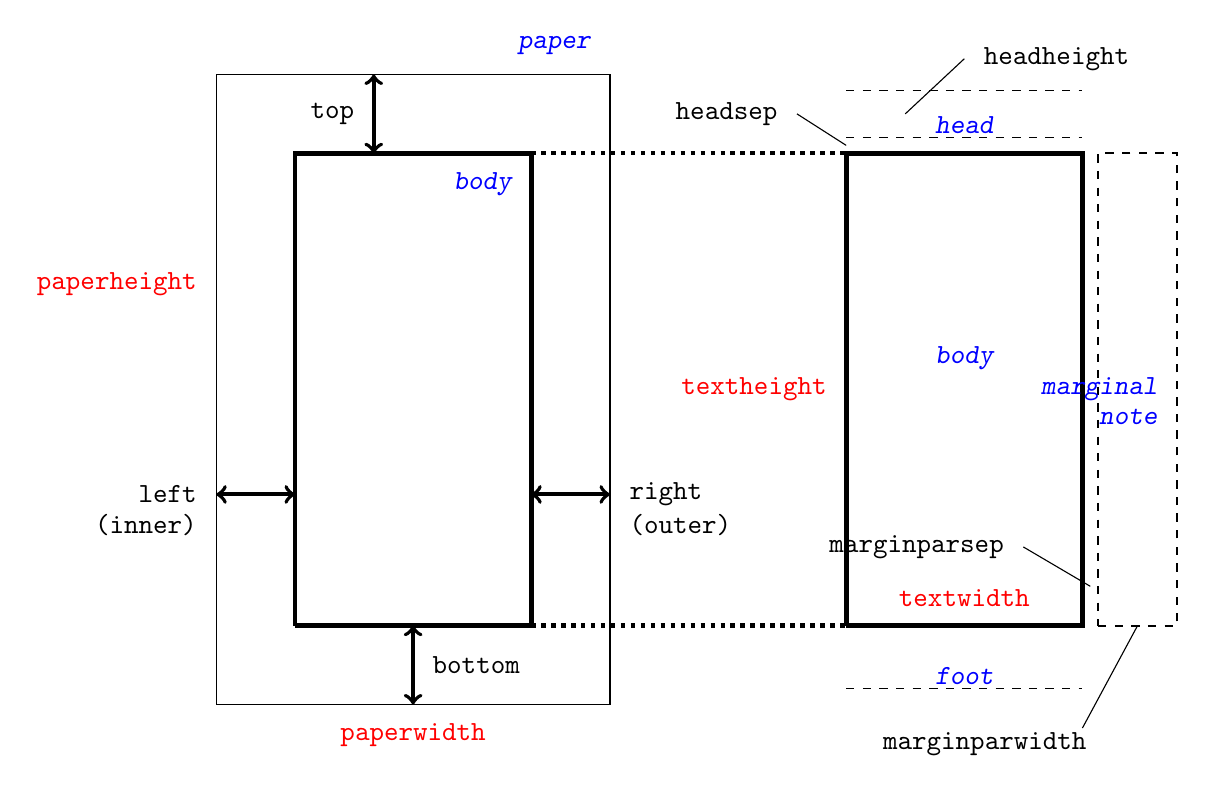
\begin{tikzpicture}{scale=0.9}
% outer-width & outer-height
\newcommand{\owd}{5};
\newcommand{\oht}{8};
% inner-width & inner-height
\newcommand{\iwd}{3};
\newcommand{\iht}{6};
% line length
\newcommand{\len}{5}

% Total Layout
\draw (0,0)--(\owd,0)--(\owd,\oht)--(0,\oht)--(0,0);
\draw[line width=0.06cm] (1,1)--(1+\iwd,1)--(1+\iwd,1+\iht)--(1,1+\iht)--(1,1);
\draw[ultra thick,dotted] (1+\iwd,1+\iht)--(\iwd+\len,1+\iht);
\draw[ultra thick,dotted] (1+\iwd,1)--(\iwd+\len,1);
% Arrow
\draw[<->,line width=0.05cm] (0,1/3*\oht)--(1,1/3*\oht);
\node[label=180:\texttt{left}] at (0,1/3*\oht){};
\node[label=225:\texttt{(inner)}] at (0,1/3*\oht){};
\draw[<->,line width=0.05cm] (1+\iwd,1/3*\oht)--(2+\iwd,1/3*\oht);
\node[label=0:\texttt{right}] at (2+\iwd,1/3*\oht){};
\node[label=315:\texttt{(outer)}] at (2+\iwd,1/3*\oht){};
\draw[<->,line width=0.05cm] (1+\iwd/2,1)--(1+\iwd/2,0);
\node[label=0:\texttt{bottom}] at (1+\iwd/2,0.5){};
\draw[<->,line width=0.05cm] (1+\iwd/3,1+\iht)--(1+\iwd/3,\oht);
\node[label=180:\texttt{top}] at (1+\iwd/3,1/2+\iht/2+\oht/2){};
% Outer Page Label
\node[label=135:\color{blue}{\ttfamily\slshape{paper}}] at (\owd,\oht){};
\node[label=225:\color{blue}{\ttfamily\slshape{body}}] at (1+\iwd,1+\iht){};

% Inner Page
\newcommand{\inn}{\iwd+\len};
\draw[line width=0.06cm] (\inn,1)--(\inn+\iwd,1)--(\inn+\iwd,1+\iht)--(\inn,1+\iht)--(\inn,1);
\node[label=180:\color{red}{\ttfamily{textheight}}] at (\inn,1+\iht/2){};
\node[label=90:\color{red}{\ttfamily{textwidth}}] at (\inn+\iwd/2,1){};
% Margin
\newcommand{\marsep}{0.2}
\newcommand{\marwd}{1}
\newcommand{\mar}{\inn+\iwd+\marsep}
\draw[thick,dashed] (\mar,1)--(\mar+\marwd,1)--(\mar+\marwd,1+\iht)--(\mar,1+\iht)--(\mar,1);
\draw (\mar-\marsep/2,1.5)--(\inn+3/4*\iwd,2);
\node[label=180:\texttt{marginparsep}] at (\inn+3/4*\iwd,2){};
\draw (\mar+\marwd/2,1)--(\inn+\iwd,-0.3);
\node[label=180:\texttt{marginparwidth}] at (\mar+\marsep/2,-0.5){};
% Foot
\draw[dashed] (\inn,0.2)--(\inn+\iwd,0.2);
\node[label=90:\color{blue}{\ttfamily\slshape{foot}}] at (\inn+\iwd/2,0){};
% Head
\draw[dashed] (\inn,1+\iht+0.8)--(\inn+\iwd,1+\iht+0.8);
\draw[dashed] (\inn,1+\iht+0.2)--(\inn+\iwd,1+\iht+0.2);
\node[label=90:\color{blue}{\ttfamily\slshape{head}}] at (\inn+\iwd/2,1+\iht){};
\draw (\inn,1+\iht+0.1)--(\inn-\len/8,1+\iht+0.5);
\node[label=180:\texttt{headsep}] at (\inn-\len/8,1+\iht+0.5){};
\draw (\inn+\iwd/4,1+\iht+0.5)--(\inn+\iwd/2,1+\iht+1.2);
\node[label=0:\texttt{headheight}] at (\inn+\iwd/2,1+\iht+1.2){};

% Total
\node[label=180:\color{red}{\ttfamily{paperheight}}] at (0,2/3*\oht){};
\node[label=270:\color{red}{\ttfamily{paperwidth}}] at (\owd/2,0){};
\node[label=\color{blue}{\ttfamily\slshape{body}}] at (\inn+\iwd/2,1+\iht/2){};
\node[label=180:\color{blue}{\ttfamily\slshape{marginal}}] at (\mar+\marwd,1+\iht/2){};
\node[label=225:\color{blue}{\ttfamily\slshape{note}}] at (\mar+\marwd,1+\iht/2){};
\end{tikzpicture}
\figcaption{页面构成示意图}
\label{fig:geo-paper}
\end{figure}

geometry宏包的具体的选项参数有:
\begin{para}
\item[paper=<papername>]: 其中纸张尺寸有[a0--a6, b0--b6, c0--c6]paper, ansi[a--e]paper, letterpaper, executivepaper, legalpaper.
\item[papersize=\{<width>,<height>\}]: 自定义尺寸。也可以单独对paperwidth或者paperheigth赋值。
\item[landscape]: 切换到横向纸张。默认的是portrait.
\end{para}

body部分分为两个概念:一个是总文本区(total body),另一个是主文本区(body). 总文本区可以由主文本区加上页眉(head)、页脚(foot)、侧页边(marginalpar)组成。默认的选项为includehead,表示总文本区包含页眉。要包括其他内容,可使用:\texttt{includefoot, includeheadfoot, includemp, includeall},以及以上各个参数将include改为ignore后的参数。

总文本区在默认状态下占纸张总尺寸的0.7,由scale=0.7控制,你也可以分别用\texttt{hscale}和\texttt{vscale}指定宽和高的占比。用具体的长度定义也是可以的,使用\texttt{(total)width}和\texttt{(total)height}定义总文本区尺寸,或者用\texttt{textwidth}和\texttt{textheight}定义主文本区的尺寸\footnote{当totalwidth和textwidth都定义时,优先采用后者的值。}。或者直接用\texttt{total=\{width,height\}, body=\{width,height\}}定义。甚至你可以用\texttt{lines=<num>}行数指定textheight。

页边的控制最为常用,分别用\texttt{left/inner, right/outer, top, bottom}来定义四向的页边。其中\texttt{inner, outer}参数只在文档的twoside参数启用时才有意义。你可以用\texttt{hmarginratio}来给定left(inner)与right(outer)页边宽的比例,默认是单页1:1、双页2:3。top和bottom之间的比由\texttt{vmarginratio}给定。你也可以用\texttt{vcentering, hcentering, centering}来指定页边比例为1:1. 在文档的左侧(内侧),可以指定装订线宽度\texttt{bindingoffset},使页边不会侵入。

页眉和页脚是位于top和bottom页边之内的文档元素。对于页眉和页脚的高度,分别使用\texttt{headheight/head, footskip/foot}参数指定。\texttt{hmargin, vmargin}来指定侧两和顶底的边距。它们到主文本区的参数分别是\texttt{headsep, footnotesep, marginparsep}. 你可以用\texttt{nohead, nofoot, nomarginpar}参数来清除总文本区中的页眉,页脚和侧页边。

对于在文档类documentclass命令中能使用的参数,geometry有不少也能做。比如\texttt{twoside, onecolumn, twocolumn}。甚至还能用文档类中不能用的\texttt{columnsep}(启用多栏分隔线)。

最后,这是几个小例子:
\begin{latex}
% 与Microsoft Word的默认样式相同:
\usepackage[hmargin=1.25in,vmargin=1in]{geometry}
% 书籍中靠书脊一侧的边距较小:
\usepackage[inner=1in,outer=1.25in]{geometry}
\end{latex}

\subsection{页眉和页脚}
主要借助fancyhdr宏包。\LaTeX 中的页眉页脚定义主要借助了两个命令,一个是\latexline{pagestyle},参数有:
\begin{para}
\item[empty] 无页眉页脚。
\item[plain] 无页眉,页脚只包含一个居中的页码。
\item[headings] 无页眉,页脚包含章/节名称与页码。
\item[myheadings] 无页眉,页脚包含页码和用户定义的信息。
\end{para}

另一个命令是\latexline{pagenumbering},与计数器一样,拥有\texttt{arabic, [Rr]oman, [Aa]lph}五种页码形式。

\pkg{fancyhdr}宏包给出了一个叫fancy的\latexline{pagestyle},将页眉和页脚分别分为左中右三个部分,分别叫\latexline{lhead}, \latexline{chead}, \latexline{rhead}, 以及类似的[lcr]foot. 页眉页脚处的横线粗细也可以定义,默认页眉为0.4pt、页脚为0pt. 下面是一个例子:
\begin{latex}
\usepackage{fancyhdr}
\pagestyle{fancy}
    \lhead{}
    \chead{}
    \rhead{\bfseries wklchris}
    \lfoot{Leftfoot}
    \cfoot{\thepage}
    \rfoot{Rightfoot}
\renewcommand{\headrulewidth}{0.4pt}
\renewcommand{\footrulewidth}{0.4pt}
\end{latex}

加载这个宏包,更多地是为了解决双页(twoside)文档的排版问题。对于双页文档,\pkg{fancyhdr}宏包给出了一套新的指令:用E, O表示单数页和双数页,L, C, R表示左中右,H, F表示页眉和页脚。其中H, F需要配合\latexline{fancyhf}命令使用。如果不使用H, F这两个参数,也可以使用\latexline{fancyhead},  \latexline{fancyfoot}两个命令代替。一个新的例子:
\begin{latex}
\fancyhead{} % 清空页眉
    \fancyhead[RO,LE]{\bfseries wklchris}
\fancyfoot{} % 清空页脚
    \fancyfoot[LE,RO]{Leftfoot}
    \fancyfoot[C]{\thepage}
    \fancyfoot[RE,LO]{Rightfoot}
\end{latex}

该宏包在定义双页文档时,采用了如下的默认设置:
\begin{latex}
\fancyhead[LE,RO]{\slshape \rightmark}
\fancyhead[LO,RE]{\slshape \leftmark}
\fancyfoot[C]{\thepage}
\end{latex}

上例中的\latexline{rightmark}表示较低级别的信息,即当前页所在的section,形式如“1.2 sectionname ”,对于article则是subsection;而\latexline{leftmark}表示较高级别的信息,即对应的chapter,对于article则是section. 命令\latexline{leftmark}包含了页面上\latexline{markboth}\footnote{\latexline{markboth}是一个会被\latexline{chapter}等命令调用的命令,默认右参数是空。注意,带星号的大纲不调用这一命令,你需要这样书写:\latexline{chapter*\{This\char`\\markboth\{This\}\{\}\}}。}下的最后一条命令的左参数,比如该页上出现了section 1--2,那么leftmark就是“Section 2”;命令\latexline{rightmark}则包含了页面上的第一个\latexline{markboth}命令的右参数或者第一个\latexline{markright}命令的唯一参数,比如可能是“Subsection 1.2”。

这听起来可能难以理解,但是\latexline{markboth}命令有两个参数,分别对应显示在文档的左页和右页(但是默认右参数留空,用\latexline{markright}去指定右页),故有左右之分;而\latexline{markright}命令只有一个参数。你可以试着再去理解一下双页文档下的宏包的默认设置。利用这一点来重定义chaptermark(book/report), sectionmark, subsectionmark(article)命令,举个例子:
\begin{latex}
% 这里的参数#1是指输入的section/chapter的标题
% 效果:“1.2. The section”
\renewcommand{\sectionmark}[1]{\markright{\thesection.\ #1}}
% 效果:“CHAPTER 2. The chapter”
\renewcommand{\chaptermark}[1]{\markboth{\MakeUppercase{%
    \chaptername}\ \thechapter.\ #1}{}}
\end{latex}

如果你对于默认的\latexline{pagestyle}不满意,可以用\latexline{fancypagestyle}命令进行更改。例如更改plain页面类型:
\begin{latex}
\fancypagestyle{plain}{
    \fancyhf{} % 清空页眉页脚
    \fancyhead[c]{\thesection}
    \fancyfoot{\thepage}}
\end{latex}

\section{抄录与代码环境}
抄录是指将键盘输入的字符(包括保留字符和空格)不经过\TeX 解释,直接输出到文档。默认的字体参数是等宽字族(ttfamily)。用法是\latexline{verb(*)}命令或者\envi{verbatim(*)}环境,区别在于带星号的会将空格以“\textvisiblespace”(\latexline{textvisiblespace})的形式标记出来。

注意,\latexline{verb}命令是一个特殊的命令,可以用一组花括号括住抄录内容,也可以任意两个同样的符号(但不能是*)。比如:
\begin{latex}
\verb|fooo{}bar|
\verb+fooo{}bar+
\end{latex}

\latexline{verb(*)}以及\envi{verbatim(*)}环境很脆弱,不能隐式地用于自定义环境,也一般不能用作命令的参数。\pkg{verbatim}宏包提供了更多的抄录支持,\pkg{fancyvrb}宏包提供了\latexline{SaveVerb}, \latexline{UseVerb}命令,以及便于实现居中的\envi{BVerbatim}环境(置于\envi{center}环境内即可),详情读者可自行查阅。

宏包\pkg{shortverb}支持以一对符号代替\latexline{verb}命令,比如竖线号:
\begin{latex}
% \usepackage{shortverb}
\MakeShortVerb|
Verbatim between this pair of verts: |#\?*^|
\end{latex}

代码环境的输出,比如本文中带行号的代码块,参见\hyperref[sec:coding]{这一节}。

\begin{multicols}{2}[\section{分栏}]
这部分内容使用文档类的\texttt{two\-column}可选参数就能实现。在\LaTeX 的双栏模式下,\latexline{newpage}命令只能进行换栏操作,而\latexline{clearpage}命令才会换进行换页操作。同时,文中随时可以使用\latexline{twocolumn}或者\latexline{onecolumn}命令执行\RED{换页、清空浮动队列,并切换分栏模式}。在双栏上方的跨栏内容,如摘要,可以写在\latexline{twocolumn[\ldots]}可选参数中。

栏之间的间距由\latexline{columnsep}控制;栏宽为\latexline{columnwidth},但请不要手工修改这个值。它可以被用作参数传递给其他命令。栏之间的分隔线宽由长度\latexline{columnseprule}给出,默认值为0pt,一般需要可以将其设置为0.4pt。 

如果在同一页内需要分栏与单栏并存,或者想要分成多栏,可以尝试使用\pkg{multicol}宏包。它提供一个支持任意多栏、但是边注和浮动体\footnote{带星号的浮动体或许可以使用,如\envi{figure*},但参数\texttt{h}会失效。}无法使用的环境。比如本节:
\begin{latex}
\begin{multicols}{2}
  [\section{分栏}]
  ...
\end{multicols}
\end{latex}

同时,该宏包会对齐每一栏的下边缘;在该环境下,使用\latexline{columnbreak}来强制切换到新的一栏。还需要指出的是,该宏包并不保证各栏之间每行的网格都是对齐的。如果你需要此功能,可以参考\pkg{grid}宏包。
\end{multicols}

\section{文档拆分}
\label{sec:include}
文档拆分只需要在主文件中使用\latexline{input\{filename.tex\}}或\latexline{include\{filename\}}命令,后者不写扩展名默认为.tex。两者区别在于\latexline{include}命令将会插入\latexline{clearpage}再读取文件。

拆分的优势在于可以根据chapter(或其他)分为多个文件,省去了长文档浏览时的一些不便。你也可以把整个导言区做成一个文件,然后在不同的\LaTeX 文档中反复使用,即充当模板的功能。你还可以把较长的tikz绘图代码写到一个tex中,在需要时\latexline{input}即可。

在导言区定义\latexline{includeonly}加上filename,可以确保只引入列表中的文件。在被引入文件的最后加入\latexline{endinput}命令,其后的内容会被忽略。

一种较规范的拆分文件的文件头,以本文的章节放在次级目录中为例:
\begin{latex}
%!TEX root = ../LaTeX-cn.tex
\end{latex}

\section{西文排版及其他}
\subsection{连写}
\LaTeX 排版以及正规排版中,如果你输入ff, fl, fi, ffi等内容,它们默认会连写。在字母中间插入空白的箱子以强制不连写:f~\latexline{mbox\{\}}~l。

\subsection{断词}
行末的英文单词太长,\LaTeX 就会以其音节断词。如果你想指定某些单词的断词位置,使用如下命令断词。例子:
\begin{latex}
\hyphenation{Hy-phen-a-tion FORTRAN}
\end{latex}

这个例子允许Hyphenation, hyphenation在短横处断词,同时\textbf{禁止}FORTRAN, Fortran, fortran断词。如果你在行文中加入\verb|\-|命令,则可以实现允许在对应位置断词的效果。比如:

\begin{codeshow}
I will show you this:
su\-per\-cal\-i\-frag\-i\-lis\-%
tic\-ex\-pi\-al\-i\-do\-cious
\end{codeshow}

如果你不想断词,比如电话号码,巧妙利用\latexline{mbox}命令吧:
\begin{latex}
My telephone number is: \mbox{012 3456 7890}
\end{latex}

\subsection{硬空格与句末标点}
如果你想在某个不带参数的命令后输入空格,请接上一个空的花括号确保空格能够正常输出。例如:\latexline{这是\char`\\TeX\{\} Live. }

在\LaTeX 中还有一个命令“\texttt{\char92\textvisiblespace}”,用于产生一个硬空格(区别于软空格\texttt{\char92space}),所以你也可以用\latexline{TeX\char`\\ \textvisiblespace Live}。

西文排版下,\LaTeX 会判断一种\co{句末标点},即小写字母后的“.”,“?”或者“!”三个英文标点。句末标点后如果键入空格,\LaTeX 会自动增加空格的距离。如果句子以大写字母结尾,\LaTeX 会认为这是人名而不增加空格,这时候需要手动添加命令\latexline{@}:

\begin{codeshow}
OK. That's fine.\\
OK\@. That's fine.
\end{codeshow}

相反,有些并非句末标点的情况会被识别为句末标点,这时候需要在标点后插入一个\latexline{\textvisiblespace}或者\verb|~|来缩小间距;区别在于前者允许断行,后者不允许。

\begin{codeshow}
Prof. Smith is a nice man.\\
Prof.~Smith is a nice man.
\end{codeshow}

在标点后使用\latexline{frenchspacing}命令,可以调整为极小的空距。这个命令在排版参考文献列表时可能被使用。

在\xelatex 编译模式下的中文字符,与西文或者符号之间会产生默认的空距\footnote{这个问题在ctex文档类下似乎被已解决。}。如果你不想要这个空距,把中文放在\latexline{mbox}内即可,比如:

\begin{codeshow}
\mbox{例子}-1
\end{codeshow}

\subsection{特殊符号}
符号的总表可以参照symbols-a4文档,运行texdoc symbols-a4即可调出。包括希腊字母在内的一些数学符号将会在下一章介绍。这里给出基于\pkg{wasysym}宏包的一些常用符号:
\begin{center}
  \centering
  \tabcaption{wasysym宏包符号}
  \begin{tabular}{*{3}{c >{\ttfamily\char92}p{5.5em}}}
     \permil     & permil   & \male     & male  & \female       & female \\
     \checked    & checked  & \XBox     & XBox  & \CheckedBox   & CheckedBox \\
     \hexstar    & hexstar  & \phone    & phone & \twonotes     & twonotes
  \end{tabular}
\end{center}
